\subsection{Das elektrische Feld meherer Punktladungen}
\begin{multicols}{2}
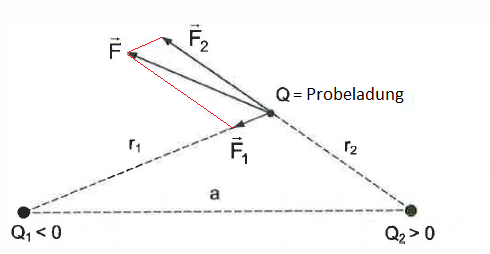
\includegraphics[width=6cm]{./pics/f_2pkt_probeladung.png} 
$\vec{F}=\vec{F_1}+\vec{F_1} = Q \cdot E_1 + Q \cdot E_2$\\
$\vec{E}= \vec{E_1} + \vec{E_2}$\\
$\vec{E}= \vec{E_1} + \vec{E_2} + \ldots + \vec{E_n} =
\sum\limits_{n}^{i=1}\vec{E_i}=\sum\limits_{n}^{i=1}\frac{Q_i}{4\pi\epsilon
{r_i}^2}\vec{e}_{ri} $\\
\end{multicols}